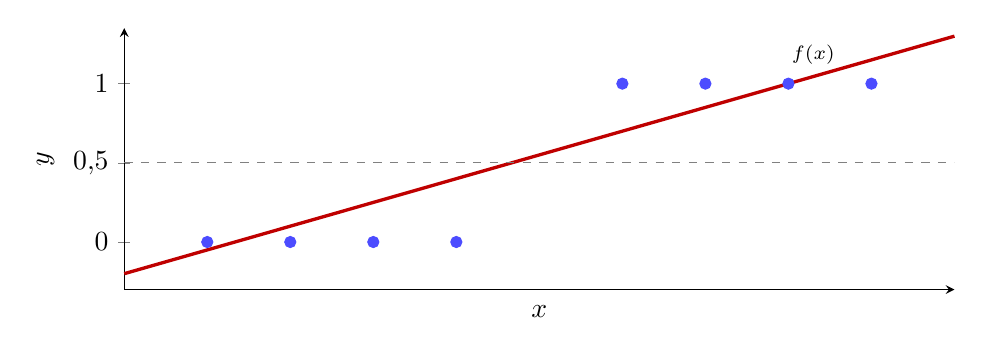
\begin{tikzpicture}
    \begin{axis}[
        width=\textwidth,
        height=4.9cm,
        xmin=0, xmax=10,
        ymin=-0.3, ymax=1.35,
        axis lines=left,
        xlabel={$x$},
        ylabel={$y$},
        xtick=\empty,
        ytick={0,0.5,1},
        yticklabels={$0$,$0{,}5$,$1$},
        clip=false
    ]
        \addplot[
            only marks,
            mark=*,
            mark size=2pt,
            blue!70
        ] coordinates {
            (1,0) (2,0) (3,0) (4,0)
            (6,1) (7,1) (8,1) (9,1)
        };

        \addplot[
            very thick,
            red!75!black,
            domain=0:10,
            samples=2
        ] {-0.2+0.15*x};

        \addplot[
            dashed,
            gray,
            domain=0:10,
            samples=2
        ] {0.5};

        \node[font=\scriptsize] at (axis cs:8.3,1.18)
            {$f(x)$};
    \end{axis}
\end{tikzpicture}
